\chapter{Background}
\section{Video Games}

Video games are a genre of digital games that has become extremely popular all over the world. There exist several different gaming consoles, and for each console there has been developed an endless amount of different games that meets almost every need and interest. Video games can be described as "electronic, interactive games known for their vibrant colors, sound effects, and complex graphics" \cite{videogamedef}. Hand held controllers or devices that capture movement are used to interact with the video game. The variety of video games makes it usable for many different purposes, like learning and education, exercising or just pure entertainment (veldig likt som oppgaven) \cite{project}. 

One might associate video games with children and teenagers, and many hours of game play, which partly is a right assumption to make. Video games are played for several hours every day, and it has taken a great part in people's everyday life. Gaming was usually associated with being anti-social, because of all the time used looked up in a room playing, but video games has emerged from sedentary, lonely gaming to gaming involving social interaction and movement. In USA in 2010, one fourth of all gamers were under the age of 18, but an interesting fact is that as much as 26 percent of the gamers are over 50 years old. This shows that not only children and teenagers uses video games, a great share of elderly has started to use this type of technology. In Norway,  as much as 8 percent of the population in the age range from 45 - 79 use computer or video games every day \cite{project}. Elderly contributes to a great share of the world's population, and if the entertainment industry could see this group as potential customers, it would open up a new and inexperienced market for video games \cite{ijsselsteijn2007digital}. 

\section{Serious Games}
The widespread and assorted use of video games have made a great potential for the entertainment industry with regard to development of new games, but also in terms of developing games for additional purposes beside pure entertainment. A new way to use video games is for different types of training, education and learning, which is called serious games. Serious games can be described as "a mental contest, played with a computer in accordance with specific rules, that uses entertainment to further government or corporate training, education, health, public policy, and strategic communication objectives" \cite{zyda2005visual}. The idea is to use the fun, motivating and captivating features that video games possess and combine it with pedagogy. Which video games to be defines as serious games depends on how the game is used, the purpose of the game and the users gaming experience. 

The term serious games is not something new, it has existed for many years, and it was introduced by the American Clark Abt in 1968 when he wrote a book about the subject. The idea of serious games started in 1950 with research on non-electronic board games for use as educational tools, and it has since then been done much research on this topic. Findings in a great amount of these research studies focus on the use of video games for educational purposes. For a video game to function as a pedagogical tool results showed that it has to focus on motivation, effectiveness, debriefing, and intuitiveness. These games have to provide motivating factors that engage students to play the game, and they have to be effective in the matter of learning outcome. Debriefing has the intention of creating a state of mind where thoughts and feelings are processed after playing the game, which is crucial aspects of learning games. When it comes to intuitiveness, students have to be able to play and understand the video games without any help from teachers. One way to engage learning is use of what is called behaviourism, which is a theory about including rewards for learning in the game play. Behaviourism has shown promise in influencing teaching and learning, and it also states that if someone is rewarded for a particular behaviour, hi or she is likely to repeat the behaviour that trigged the reward \cite{behaviour}. In the 1980s there was an increased focus on development of cognitive skills. This combined with the principles of behaviourism was called an instructional approach. This is based on principles related to exercise and reward, which is that repeated exercise is crucial to acquire new knowledge, and that willingness to learn could be encouraged by rewards. Instructional behaviour also says something about how video games in the best possible way can influence players, and how to handle difficulties related to learning. This could be difficulties like concentration, slow adoption of knowledge, and motivation. Intrinsic motivation is an important aspect in good educational games, and to achieve this, elements like fantasy, control, challenge and curiosity should be included. The first serious attempt in developing video games with the main focus on learning did not become very successful \cite{understandingvg}. The failure that time was that the focus in these  video games were on pure learning, which resulted in boring games that did not create motivation and curiosity \cite{understandingvg} \cite{susi2007serious}. Michael Zyda states that, in serious games, pedagogy has to be subordinate to the story and entertainment component of the game. It is highly important that fun and entertainment is the main focus in the game \cite{zyda2005visual}

There exist several genres of serious games, where edutainment and game-based learning, advertaintment, games for politics, simulation games, and games for health are some of them. The genre of edutainment and game-based learning combines fun and entertainment with education and learning. Advertainment is about using video games as a media for marketing, and games for politics uses video games to influence players through hidden, underlying political messages. Simulation games is about bringing various activities into life with the use of video games, and gaming for health is use of video games to engage activity, to become physically stronger, and to improve quality of life. Gaming for health includes a topic called exercise games, which has training as a main focus \cite{understandingvg} \cite{alfingewang}.

An already mentioned feature with serious games is that they provide the opportunity to experience real-life situations and adventures one may otherwise not be able to enjoy. This might be due to expenses, time, distance, risk, or physical capabilities. With serious games it is possible to play golf, be the star of a boxing match, paddle down turbulent rivers, and explore nature and creatures one have never seen before. In a more serious matter, video games can be used to simulate brain surgery or a battle in a war zone. This can teach students how to perform medical procedures or it could prepare soldiers for war. Serious games can also be used for students to learn their curriculum through quiz games, and people can be motivated to work out with exercise games. Serious games can be used in several situations, and for purposes, and it can help people develop a huge number of different skills. 

Research on use of serious games shows positive development of skills and knowledge, in addition to positive effect on health, which results in motivation for further research and development. In addition, the new technology involving physical interfaces and improvement on graphics and animations initiates to new types of games. The market for serious games are inexperienced and unexplored, so there are a great potential for further research \cite{alfingewang}. Market sales the last couple of years also shows promise for serious video games in the future. In 2008, the market for serious games sold for around 1,5 billion USD around the globe \cite{alfingewang}, and in 2010 it reached about 2 billion USD (1,5 billion EUR). The market is expecting a annual growth rate of 47 percent, up to impressive 13,5 billion USD (10 billion EUR) in 2015 \cite{idate}. 

We will look deeper into one of the genres within serious games, exercise games.  

\section{Exergames}
Exercise games, or exergames, is a type of serious video games that combines the traditional game play with physical activity. The combination of required movement and amusement is used to stimulate exercise and engage people to be more physically active in a more fun and motivating way. Much research has been done in the area of exergames, and results show that exergames can have a positive effect on users health. In addition to being a new, fun and different way to work out, exergames provide an opportunity for social interaction. A great amount of today’s existing computer and video games possess this feature, and as much as 78 percent of all gamers say they play with others either in-person or online. One of the two top-selling video games in 2011 was Just Dance 3, which is an exergame that has the possibility to play with others \cite{statistics2012}. This shows that the social aspect of gaming is important for the players. The social aspect these games provide may also be especially important for people who experience loneliness in their everyday life \cite{project}.

Exergames uses technology like remote hand held controllers and motion sensors which capture body movement. Users are therefore required to get up and move their body to be able to play the game. There exist several consoles that support this technology, where Nintendo Wii, Playstation Move, Dance Dance Revolution and Xbox Kinect are some of them. The existing consoles uses different type of devices to capture body movement, like hand held controllers, different boards and pads with embedded sensors, and video cameras with motion sensors. In this assignment we will focus on the Kinect sensor technology. 

\section{Microsoft Kinect for Xbox 360 and Windows}
Microsoft Kinect is a motion sensor that captures movement without the use of any controllers. This gives players the opportunity to play and interact with the game only by gestures and body movement. Xbox presents the Kinect experience this way, "Kinect for Xbox 360 brings games and entertainment to life in extraordinary new ways without using a controller" \cite{kinectxboxdef}. The word Kinect is a fusion of two words, \emph{kinetic}, which means movement, and \emph{connect}, which is meant to relate to the social aspect \cite{howstuffworksKinect}. The Kinect sensor was released by Microsoft in November 2012 as an input device to the Xbox 360 console, and it did not take long before the Microsoft Kinect got extremely popular. Only ten days after the release in 2010 it had been sold 1 million Kinect motion sensors, and in January 2012, sales numbers had climbed up to over 18 million sold units \cite{kinectsales}. These sales numbers put Kinect into history, as no other consumer electronic device has experienced such great sales numbers in so short time. The Kinect sensor has the possibility to be used without the Xbox 360 console, as it also is compatible with Windows computers. To be able to use the Kinect for Windows, a Kinect sensor and a Kinect for Windows application is needed, in addition to a computer running Windows 7, Windows 8, Windows Embedded Standard 7, or Windows Embedded POSReady 7 \cite{kinectforwindows}. Microsoft has also opened up the opportunity for a third party to develop Kinect for Windows applications, by releasing a Kinect for Windows \ac{sdk} \cite{kinectforwindows}. The first \ac{sdk} was for non-commercial project, but later Microsoft also released a \ac{sdk} for commercial use. 

\begin{figure} [ht!]
\centering
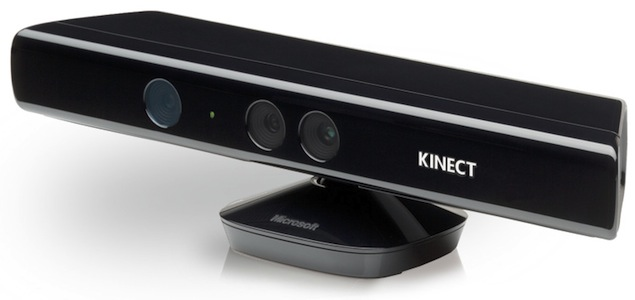
\includegraphics[scale=0.4]{kinect.jpg}
\caption{The Kinect sensor}
\label{kinectsensor}
\end{figure} 
 
Kinect has not just experienced success as an entertainment device within the living room, researches has also started to see the possibility to use the Kinect for other non-gaming purposes, e.g. within healthcare, education and industry. A key reason for the broad use of Kinect is because of its accessibility and low price, in addition to the ground breaking technology it provides. The release of the Kinect for Windows \ac{sdk} is also a reason for the wealth of non-gaming applications, as it makes the the Kinect technology available for everyone to use. http://www.microsoft.com/en-us/news/features/2011/oct11/10-31kinecteffect.aspx

We will now describe the technology the Kinect sensor provides.     

\subsection{The Kinect Sensor Technology}
The Kinect sensor is a device that captures the movement of your body and translates it into the video game. It is a oblong, black box placed a small platform, see Figure \ref{kinectsensor}. While playing, the Kinect should be placed near the TV, connected to the Xbox through a USB-port.   

In addition to capturing body movement, the Kinect sensor is also able to recognise both a player's face and voice.

The Kinect sensor consist of a trio of hardware; a depth sensor, a RGB video camera and multi-array microphones. The depth sensor is a composition of a one-colored sensor and an infrared projector. These to elements together make it possible to measure distance of elements and to see the room in 3D. The video camera captures the three colors red, green and blue (RGB), and it uses these colors to detect faces and other features. In the Kinect sensor there is four microphones, aligned in an array. These microphones separates voice from noise, which makes it possible to stand a certain distance from the sensor and still have the Kinect sensor recognising your voice.          

Litt mer generelt om Kinect
Hva som gjør teknologien mulig, hva består sensoren av.
Snakke litt om face recognition. 